\documentclass{standalone}
\usepackage{tikz}
\usetikzlibrary{%                                                               
  shapes,arrows,positioning,decorations.markings,matrix,fit,tikzmark,           
  shapes.geometric,calc}
\tikzstyle{line} = [draw, -latex',line width=.7pt,fill=none]
\tikzstyle{dline} = [draw, latex'-latex',line width=.7pt,fill=none]
\definecolor{mBlue}{RGB}{4,110,152}
\definecolor{mGreen}{RGB}{115,180,85}
\definecolor{mYellow}{RGB}{230,195,35}
\definecolor{mOrange}{HTML}{EB811B}
\pgfdeclarelayer{background}
\pgfdeclarelayer{foreground}
\pgfsetlayers{background,main,foreground}
\begin{document}
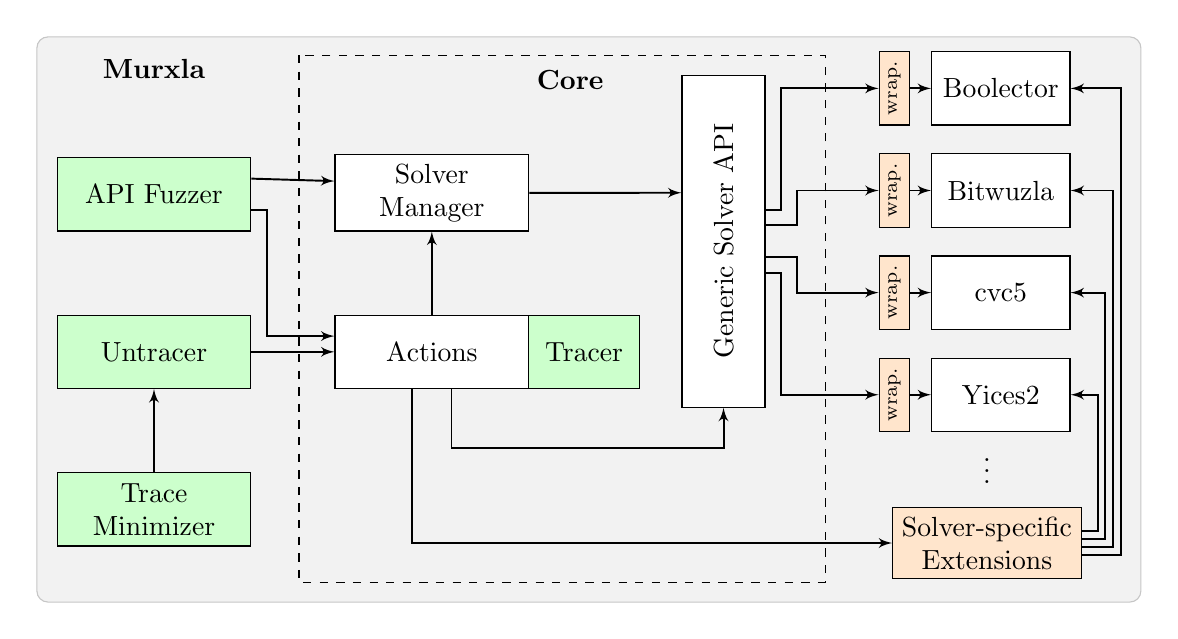
\begin{tikzpicture}[
    block/.style={
      draw,
      minimum width=7em,
      minimum height=2.65em,
      fill=white,
      align=center
    },
    component/.style={
      draw,
      minimum width=7em,
      minimum height=2.65em,
      fill=green!20,
      align=center
    },
    solver/.style={
      draw,
      minimum height=2.65em,
      minimum width=5em,
      fill=white,
    },
    solverimpl/.style={
      draw,
      minimum height=2.65em,
      fill=orange!20
    },
    ext/.style={
      draw,
      fill=orange!20,
      align=center
    }
  ]

  \node[component] (fsm) {API Fuzzer};
  \node[component,below=3em of fsm] (untracer) {Untracer};
  \node[component,below=3em of untracer] (dd) {Trace\\Minimizer};

  \node[above=2.5em of fsm] (title) {\textbf{Murxla}};

  \node[block,right=3em of untracer] (actions) {Actions};
  \node[component,minimum width=4em,right=-\pgflinewidth of actions] (tracer) {Tracer};

  \node[block,above=3em of actions] (slvmgr) {Solver\\Manager};

  \node[block,right=1.5em of tracer,minimum height=12em,minimum width=3em,yshift=4em] (api) {\rotatebox{90}{Generic Solver API}};

  \node[solver,right=7.5em of api.north,yshift=-.5em] (btor) {Boolector};
  \node[solverimpl, left=.75em of btor] (btori) {\rotatebox{90}{\scriptsize wrap.}};
  \draw[line] (btori) -- (btor);

  \node[solver,below=1em of btor] (bzla) {Bitwuzla};
  \node[solverimpl, left=.75em of bzla] (bzlai) {\rotatebox{90}{\scriptsize wrap.}};
  \draw[line] (bzlai) -- (bzla);

  \node[solver,below=1em of bzla] (cvc) {cvc5};
  \node[solverimpl, left=.75em of cvc] (cvci) {\rotatebox{90}{\scriptsize wrap.}};
  \draw[line] (cvci) -- (cvc);

  \node[solver,below=1em of cvc] (yices) {Yices2};
  \node[solverimpl, left=.75em of yices] (yicesi) {\rotatebox{90}{\scriptsize wrap.}};
  \draw[line] (yicesi) -- (yices);

  \node[below=0em of yices,xshift=-.5em] (others) {\vdots};

  \node[ext,below=.5em of others] (ext) {Solver-specific\\Extensions};



  \draw[line] (dd) -- (untracer);

  \draw[line] (untracer) -- (actions);
  \draw[line] (fsm.east)+(0,-.2) -- +(0.2,-.2) |- ($(actions.west)+(0,.2)$);
  \draw[line] (fsm.east)+(0,.2) -- ($(slvmgr.west)+(0,.15)$);

  \draw[line] (actions) -- (slvmgr);
  \draw[line] (actions.south)+(0.25,0) |- +(0.25,-0.75) -| (api.south);
  \draw[line] (actions.south)+(-0.25,0) |- (ext);

  \draw[line] (slvmgr) -- (api.131);

  \draw[line] (api.east)+(0,.4) -- +(.2,.4) |- (btori);
  \draw[line] (api.east)+(0,.2) -- +(.4,.2) |- (bzlai);
  \draw[line] (api.east)+(0,-.2) -- +(.4,-.2) |- (cvci);
  \draw[line] (api.east)+(0,-.4) -- +(.2,-.4) |- (yicesi);

  \draw[line] (ext.east)+(0,-.15) -- +(.5,-.15) |- (btor.east);
  \draw[line] (ext.east)+(0,-.05) -- +(.4,-.05) |- (bzla.east);
  \draw[line] (ext.east)+(0,.05) -- +(.3,.05) |- (cvc.east);
  \draw[line] (ext.east)+(0,.15) -- +(.2,.15) |- (yices.east);

  \node[above=2em of slvmgr,xshift=5em] (core) {\textbf{Core}};

  \begin{pgfonlayer}{background}
    \path (fsm.west)+(-0.25,2) node (c0) {};
    \path (ext.east)+(.75,-0.75) node (c1) {};
    \path[rounded corners, draw=gray!45, fill=gray!10] (c0) rectangle (c1);
  \end{pgfonlayer}

  \begin{pgfonlayer}{foreground}
    \path (slvmgr.west)+(-0.45,1.75) node (c0) {};
    \path (ext.west)+(-.85,-.5) node (c1) {};
    \draw[dashed] (c0) rectangle (c1);
  \end{pgfonlayer}

\end{tikzpicture}%
\end{document}
